% questions.tex —— 2015 年·重庆卷·文史类 · 题目内容片段（无答案）
% 由 tools/generate_projects.py 依来源总账自 2015/2015_数学真题_重庆文_试题.md 生成，勿手改（改源 MD 后重跑）


\begin{gktip}
来源说明：固定源为 2 页 A3 扫描件，印刷页 941–942，卷内无答案。卷首无注意事项框，卷面亦无「第Ⅰ卷/第Ⅱ卷」字样，均照录不补。第 5 题题干扫描止于「体积」，未见「为」字，照录。

图形说明：第 4、5、8、20、21 题图依原页拓扑重绘，不按比例。
\end{gktip}

\begin{gktip}
卷面抬头：2015 普通高等学校招生考试（重庆卷文）

（源疑点：扫描件卷首只有上述标题行，其后直接为「一、选择题」，没有注意事项说明框，也没有「第Ⅰ卷」「第Ⅱ卷」字样；两页页脚印刷页码分别为 941、942。此处照扫描页记录，未按常见卷式补写。）

（源疑点：第 5 题题干在扫描页上止于「则该几何体的体积」，其后直接为选项，未见「为」字；此处照录，未补字。）
\end{gktip}

\gkpart{一、选择题}

\begin{question}
\gkti{1}已知集合 $A=\{1,2,3\}$，$B=\{1,3\}$，则 $A\cap B=$（　）。

（A）$\{2\}$；（B）$\{1,2\}$；（C）$\{1,3\}$；（D）$\{1,2,3\}$。

\end{question}
\begin{question}
\gkti{2}“$x=1$”是“$x^{2}-2x+1=0$”的（　）。

（A）充要条件；（B）充分而不必要条件；（C）必要而不充分条件；（D）既不充分也不必要条件。

\end{question}
\begin{question}
\gkti{3}函数 $f(x)=\log_{2}(x^{2}+2x-3)$ 的定义域是（　）。

（A）$[-3,1]$；（B）$(-3,1)$；（C）$(-\infty,-3]\cup[1,+\infty)$；（D）$(-\infty,-3)\cup(1,+\infty)$。

\Needspace{0.4\textheight}
\end{question}
\begin{question}
\gkti{4}重庆市 $2013$ 年各月的平均气温（$^\circ$C）数据的茎叶图如下：
\nopagebreak[4]
\begin{center}% 2015 年重庆卷（文史类）第 4 题：平均气温数据的茎叶图（依固定扫描页重绘，只画拓扑与标号，不按比例）
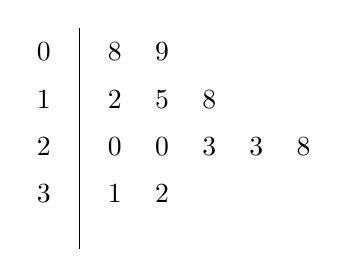
\begin{tikzpicture}[scale=1.0]
  % 茎叶分隔线
  \draw (0,2.55)--(0,-0.25);
  % 茎 0
  \node at (-0.45,2.25) {$0$};
  \node at (0.45,2.25) {$8$};
  \node at (1.05,2.25) {$9$};
  % 茎 1
  \node at (-0.45,1.65) {$1$};
  \node at (0.45,1.65) {$2$};
  \node at (1.05,1.65) {$5$};
  \node at (1.65,1.65) {$8$};
  % 茎 2
  \node at (-0.45,1.05) {$2$};
  \node at (0.45,1.05) {$0$};
  \node at (1.05,1.05) {$0$};
  \node at (1.65,1.05) {$3$};
  \node at (2.25,1.05) {$3$};
  \node at (2.85,1.05) {$8$};
  % 茎 3
  \node at (-0.45,0.45) {$3$};
  \node at (0.45,0.45) {$1$};
  \node at (1.05,0.45) {$2$};
\end{tikzpicture}
\end{center}
\nopagebreak[4]
则这组数据的中位数是（　）。

（A）$19$；（B）$20$；（C）$21.5$；（D）$23$。

\Needspace{0.4\textheight}
\end{question}
\begin{question}
\gkti{5}某几何体的三视图如图所示，则该几何体的体积（　）。
\nopagebreak[4]
\begin{center}% 2015 年重庆卷（文史类）第 5 题：某几何体的三视图（依固定扫描页重绘，只画拓扑与标号，不按比例）
\begin{tikzpicture}[>=stealth,scale=1.0]
  % 正视图：边长 2 的正方形，左下接直角三角形（水平边 1、竖直边 1）
  \draw (0,0) rectangle (2,2);
  \draw (-1,1)--(0,1)--(0,0)--cycle;
  % 正视图尺寸标注
  \draw[<->] (-1,1.45)--(0,1.45);
  \node at (-0.5,1.72) {$1$};
  \draw[<->] (0.28,1)--(0.28,2);
  \node at (0.62,1.5) {$1$};
  \draw[<->] (0.28,0)--(0.28,1);
  \node at (0.62,0.5) {$1$};
  \node at (0.5,-0.55) {正视图};
  % 左视图：半径 1 的圆，水平直径
  \draw (4.5,1) circle (1);
  \draw (3.5,1)--(5.5,1);
  \node at (4.5,-0.55) {左视图};
  % 俯视图：边长 2 的正方形，左侧接等腰三角形（底 2、高 1）
  \draw (0,-4) rectangle (2,-2);
  \draw (-1,-3)--(0,-2)--(0,-4)--cycle;
  % 俯视图尺寸标注
  \draw[<->] (2.35,-2)--(2.35,-4);
  \node at (2.72,-3) {$2$};
  \draw[<->] (0,-4.4)--(2,-4.4);
  \node at (1,-4.7) {$2$};
  \node at (0.5,-5.25) {俯视图};
\end{tikzpicture}
\end{center}
\nopagebreak[4]
（A）$\dfrac{1}{3}+2\pi$；（B）$\dfrac{13\pi}{6}$；（C）$\dfrac{7\pi}{3}$；（D）$\dfrac{5\pi}{2}$。

\end{question}
\begin{question}
\gkti{6}若 $\tan\alpha=\dfrac{1}{3}$，$\tan(\alpha+\beta)=\dfrac{1}{2}$，则 $\tan\beta=$（　）。

（A）$\dfrac{1}{7}$；（B）$\dfrac{1}{6}$；（C）$\dfrac{5}{7}$；（D）$\dfrac{5}{6}$。

\end{question}
\begin{question}
\gkti{7}已知非零向量 $\boldsymbol{a}$，$\boldsymbol{b}$ 满足 $|\boldsymbol{b}|=4|\boldsymbol{a}|$，且 $\boldsymbol{a}\perp(2\boldsymbol{a}+\boldsymbol{b})$，则 $\boldsymbol{a}$ 与 $\boldsymbol{b}$ 的夹角为（　）。

（A）$\dfrac{\pi}{3}$；（B）$\dfrac{\pi}{2}$；（C）$\dfrac{2\pi}{3}$；（D）$\dfrac{5\pi}{6}$。

\Needspace{0.4\textheight}
\end{question}
\begin{question}
\gkti{8}执行如图所示的程序框图，则输出 $s$ 的值为（　）。
\nopagebreak[4]
\begin{center}% 2015 年重庆卷（文史类）第 8 题：程序框图（依固定扫描页重绘，只画拓扑与标号，不按比例）
\begin{tikzpicture}[>=stealth,scale=0.85]
  % 开始
  \draw[rounded corners=6pt] (-1.0,11.6) rectangle (1.0,12.4);
  \node at (0,12.0) {开始};
  \draw[->] (0,11.6)--(0,11.2);
  % 赋初值
  \draw (-1.8,10.4) rectangle (1.8,11.2);
  \node at (0,10.8) {$s=0,\ k=0$};
  \draw[->] (0,10.4)--(0,9.9);
  % 判断 k<8
  \draw (-1.9,7.4)--(0,6.7)--(1.9,7.4)--(0,8.1)--cycle;
  \node at (0,7.4) {$k<8$};
  \draw[->] (0,9.9)--(0,8.1);
  % 否
  \draw[->] (0,6.7)--(0,6.0);
  \node at (0.35,6.35) {否};
  \draw (-1.4,6.0)--(1.4,6.0)--(1.2,5.2)--(-1.6,5.2)--cycle;
  \node at (-0.1,5.6) {输出 $s$};
  \draw[->] (0,5.2)--(0,4.6);
  \draw[rounded corners=6pt] (-1.0,4.6) rectangle (1.0,3.8);
  \node at (0,4.2) {结束};
  % 是：先 k=k+2，再 s=s+1/k，回到判断框上方
  \draw[->] (1.9,7.4)--(4.6,7.4)--(4.6,7.9);
  \node at (2.5,7.65) {是};
  \draw (3.5,7.9) rectangle (5.7,8.7);
  \node at (4.6,8.3) {$k=k+2$};
  \draw[->] (4.6,8.7)--(4.6,9.1);
  \draw (3.4,9.1) rectangle (5.8,9.9);
  \node at (4.6,9.5) {$s=s+\frac{1}{k}$};
  \draw[->] (4.6,9.9)--(4.6,10.2)--(0,10.2);
\end{tikzpicture}
\end{center}
\nopagebreak[4]
（A）$\dfrac{3}{4}$；（B）$\dfrac{5}{6}$；（C）$\dfrac{11}{12}$；（D）$\dfrac{25}{24}$。

\end{question}
\begin{question}
\gkti{9}设双曲线 $\dfrac{x^{2}}{a^{2}}-\dfrac{y^{2}}{b^{2}}=1$（$a>0$，$b>0$）的右焦点是 $F$，左、右顶点分别是 $A_{1}$，$A_{2}$，过 $F$ 作 $A_{1}A_{2}$ 的垂线与双曲线交于 $B$，$C$ 两点．若 $A_{1}B\perp A_{2}C$，则该双曲线的渐近线的斜率为（　）。

（A）$\pm\dfrac{1}{2}$；（B）$\pm\dfrac{\sqrt{2}}{2}$；（C）$\pm1$；（D）$\pm\sqrt{2}$。

\end{question}
\begin{question}
\gkti{10}若不等式组

\nopagebreak[4]
\[
\begin{cases}
x+y-2\le 0,\\
x+2y-2\ge 0,\\
x-y+2m\ge 0
\end{cases}
\]

表示的平面区域为三角形，且其面积等于 $\dfrac{4}{3}$，则 $m$ 的值为（　）。

（A）$-3$；（B）$1$；（C）$\dfrac{4}{3}$；（D）$3$。

\end{question}
\gkpart{二、填空题}

\begin{question}
\gkti{11}复数 $(1+2\mathrm{i})\mathrm{i}$ 的实部为\gkblank{}．

\end{question}
\begin{question}
\gkti{12}若点 $P(1,2)$ 在以坐标原点为圆心的圆上，则该圆在点 $P$ 处的切线方程为\gkblank{}．

\end{question}
\begin{question}
\gkti{13}设 $\triangle ABC$ 的内角 $A$，$B$，$C$ 的对边分别为 $a$，$b$，$c$，且 $a=2$，$\cos C=-\dfrac{1}{4}$，$3\sin A=2\sin B$，则 $c=$\gkblank{}．

\end{question}
\begin{question}
\gkti{14}设 $a$，$b>0$，$a+b=5$，则 $\sqrt{a+1}+\sqrt{b+3}$ 的最大值为\gkblank{}．

\end{question}
\begin{question}
\gkti{15}在区间 $[0,5]$ 上随机地选择一个数 $p$，则方程 $x^{2}+2px+3p-2=0$ 有两个负根的概率为\gkblank{}．

\end{question}
\gkpart{三、解答题}

\begin{question}
\gkti{16}已知等差数列 $\{a_{n}\}$ 满足 $a_{3}=2$，前 $3$ 项和 $S_{3}=\dfrac{9}{2}$．

（1） 求 $\{a_{n}\}$ 的通项公式；

（2） 设等比数列 $\{b_{n}\}$ 满足 $b_{1}=a_{1}$，$b_{4}=a_{15}$，求 $\{b_{n}\}$ 的前 $n$ 项和 $T_{n}$．

\end{question}
\begin{question}
\gkti{17}随着我国经济的发展，居民的储蓄存款逐年增长．设某地区城乡居民人民币储蓄存款（年底余额）如下表：

\begin{center}
\begin{tabular}{llllll}
\toprule
年份 & 2010 & 2011 & 2012 & 2013 & 2014 \\
\midrule
时间代号 $t$ & 1 & 2 & 3 & 4 & 5 \\
储蓄存款 $y$（千亿元） & 5 & 6 & 7 & 8 & 10 \\
\bottomrule
\end{tabular}
\end{center}

（1） 求 $y$ 关于 $t$ 的回归方程 $\hat{y}=\hat{b}t+\hat{a}$；

（2） 用所求回归方程预测该地区 $2015$ 年（$t=6$）的人民币储蓄存款．

附：回归方程 $\hat{y}=\hat{b}t+\hat{a}$ 中，$\hat{b}=\dfrac{\sum\limits_{i=1}^{n}t_{i}y_{i}-n\bar{t}\bar{y}}{\sum\limits_{i=1}^{n}t_{i}^{2}-n\bar{t}^{2}}$，$\hat{a}=\bar{y}-\hat{b}\bar{t}$．

\end{question}
\begin{question}
\gkti{18}已知函数 $f(x)=\dfrac{1}{2}\sin 2x-\sqrt{3}\cos^{2}x$．

（1） 求 $f(x)$ 的最小正周期和最小值；

（2） 将函数 $f(x)$ 的图象上每一点的横坐标伸长到原来的两倍，纵坐标不变，得到函数 $g(x)$ 的图象，当 $x\in\left[\dfrac{\pi}{2},\pi\right]$ 时，求 $g(x)$ 的值域．

\end{question}
\begin{question}
\gkti{19}已知函数 $f(x)=ax^{3}+x^{2}$（$a\in\mathbf{R}$）在 $x=-\dfrac{4}{3}$ 处取得极值．

（1） 确定 $a$ 的值；

（2） 若 $g(x)=f(x)\mathrm{e}^{x}$，讨论 $g(x)$ 的单调性．

\Needspace{0.4\textheight}
\end{question}
\begin{question}
\gkti{20}如图，三棱锥 $P-ABC$ 中，平面 $PAC\perp$ 平面 $ABC$，$\angle ABC=\dfrac{\pi}{2}$，点 $D$，$E$ 在线段 $AC$ 上，且 $AD=DE=EC=2$，$PD=PC=4$，点 $F$ 在线段 $AB$ 上，且 $EF\parallel BC$．

（1） 证明：$AB\perp$ 平面 $PFE$；

（2） 若四棱锥 $P-DFBC$ 的体积为 $7$，求线段 $BC$ 的长．
\nopagebreak[4]
\begin{center}% 2015 年重庆卷（文史类）第 20 题：三棱锥 P-ABC 与截面 PFE（依固定扫描页重绘，只画拓扑与标号，不按比例）
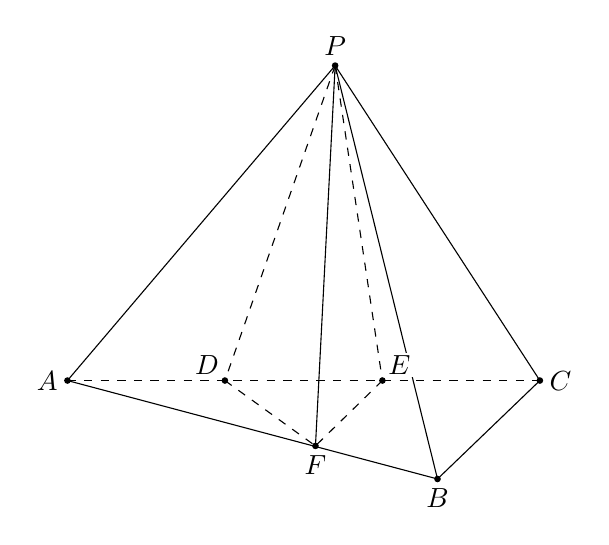
\begin{tikzpicture}[>=stealth,scale=1.0]
  % 顶点与底面各点
  \coordinate (P) at (3.4,4.0);
  \coordinate (A) at (0,0);
  \coordinate (C) at (6,0);
  \coordinate (B) at (4.7,-1.25);
  \coordinate (D) at (2,0);
  \coordinate (E) at (4,0);
  \coordinate (F) at (3.15,-0.83);
  % 实线棱
  \draw (P)--(A);
  \draw (P)--(B);
  \draw (P)--(C);
  \draw (P)--(F);
  \draw (A)--(B);
  \draw (B)--(C);
  % 虚线：AC 及内部线段
  \draw[dashed] (A)--(C);
  \draw[dashed] (P)--(D);
  \draw[dashed] (P)--(E);
  \draw[dashed] (D)--(F);
  \draw[dashed] (E)--(F);
  % 标号
  \fill (P) circle (1.2pt) node[above] {$P$};
  \fill (A) circle (1.2pt) node[left] {$A$};
  \fill (B) circle (1.2pt) node[below] {$B$};
  \fill (C) circle (1.2pt) node[right] {$C$};
  \fill (D) circle (1.2pt) node[fill=white,inner sep=1pt,above left=1pt] {$D$};
  \fill (E) circle (1.2pt) node[fill=white,inner sep=1pt,above right=1pt] {$E$};
  \fill (F) circle (1.2pt) node[below] {$F$};
\end{tikzpicture}
\end{center}
\nopagebreak[4]
\Needspace{0.4\textheight}
\end{question}
\begin{question}
\gkti{21}如图，椭圆 $\dfrac{x^{2}}{a^{2}}+\dfrac{y^{2}}{b^{2}}=1$（$a>b>0$）的左、右焦点分别为 $F_{1}$，$F_{2}$，过 $F_{2}$ 的直线交椭圆于 $P$，$Q$ 两点，且 $PQ\perp PF_{1}$．

（1） 若 $|PF_{1}|=2+\sqrt{2}$，$|PF_{2}|=2-\sqrt{2}$，求椭圆标准方程；

（2） 若 $|PQ|=\lambda|PF_{1}|$，且 $\dfrac{3}{4}\le\lambda<\dfrac{4}{3}$，试确定椭圆离心率 $e$ 的取值范围．
\nopagebreak[4]
\begin{center}% 2015 年重庆卷（文史类）第 21 题：椭圆与过右焦点的弦 PQ（依固定扫描页重绘，只画拓扑与标号，不按比例）
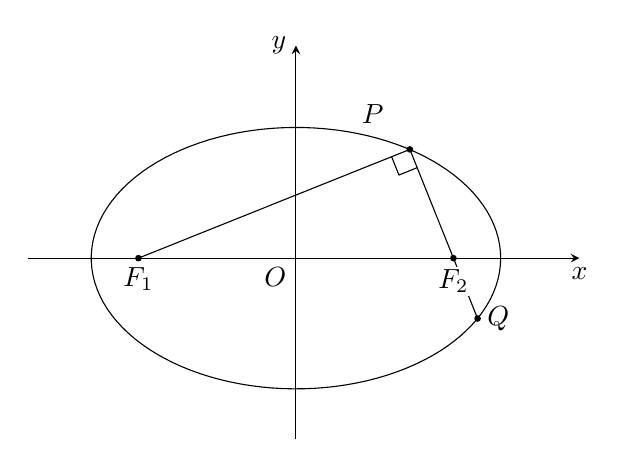
\begin{tikzpicture}[>=stealth,scale=1.0]
  % 坐标轴
  \draw[->] (-3.4,0)--(3.6,0) node[below] {$x$};
  \draw[->] (0,-2.3)--(0,2.7) node[left] {$y$};
  \node[below left] at (0,0) {$O$};
  % 椭圆 x^2/2.6^2 + y^2/1.66^2 = 1
  \draw[domain=0:360,samples=120] plot ({2.6*cos(\x)},{1.66*sin(\x)});
  % 焦点与点
  \coordinate (F1) at (-2,0);
  \coordinate (F2) at (2,0);
  \coordinate (P) at (1.447,1.381);
  \coordinate (Q) at (2.307,-0.767);
  % 弦 PQ 与线段 PF1
  \draw (P)--(Q);
  \draw (P)--(F1);
  % 直角标记（PF1 与 PQ 在 P 处）
  \draw (1.215,1.288)--(1.308,1.056)--(1.540,1.149);
  % 标号
  \fill (F1) circle (1.2pt) node[below] {$F_{1}$};
  \fill (F2) circle (1.2pt) node[fill=white,inner sep=1pt,below=3pt] {$F_{2}$};
  \fill (P) circle (1.2pt) node[above left=6pt] {$P$};
  \fill (Q) circle (1.2pt) node[right] {$Q$};
\end{tikzpicture}
\end{center}
\nopagebreak[4]

\end{question}